\documentclass[xetex,mathserif,serif]{beamer}
\usepackage{xeCJK}%preamble part
\usepackage{graphicx}
\usepackage{subcaption}
\usepackage{amsmath}
\DeclareMathOperator*{\argmax}{argmax}
\setCJKmonofont{SimSun}
\setmainfont{Times New Roman}
\setbeamertemplate{frametitle}[default][center]
\setbeamertemplate{footline}[frame number]
\begin{document}
\title[Crisis] % (optional, only for long titles)
{Rasch Model and its Application in Word Memorization Software}
%\subtitle{Evidence from India}
\author[Author, Anders] % (optional, for multiple authors)
{Zhao Feng}
\institute[Universities Here and There] % (optional)
{
  Institute of Mathematics\\
  Tsinghua University
}
%\date[KPT 2004] % (optional)
%{Conference on Presentation Techniques, 2004}
%\subject{Computer Science}
\frame{\titlepage}
  \begin{frame}
    
    %Content goes here
    在心理测试中,IRT(Item Response Theory)对某个person的能力值$\theta$(latent variable )的估计值,是通过该person在若干个item的测试结果给出的,以下的讨论局限于每个item的测试结果是0或1,分别代表答案错误与正确。假设各个item彼此独立,被试者对某个item的回答正确的概率用IRF(item response function)建模.一般能力$\theta$会做一个归一化,使得其均值为0标准差为1,这样$\hat{\theta}$作为$\theta$的估计值一般在-3到3之前,非常接近0表示水平中等。这种归一化给不同测试集之间相互比较提供了方便。
  \end{frame}
  \begin{frame}
    
    IRF函数有多种不同的建模方式,一般常用Logistic function:
\pause\begin{equation}
p_i(\theta)=c_i+\frac{1-c_i}{1+exp(-a_i(\theta-b_i))}
\end{equation}
上式中i表示被试者的编号,a,b,c是item的参数,分别表征discrimination,difficulty和pseudo guessing,可以从下图(ICC曲线,item characteristic curve)形象地说明这三个参数
\begin{figure}[!ht]
\caption{三个参数的IRF}
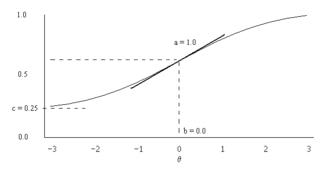
\includegraphics[height=1.5in]{3PL_IRF.png}
\end{figure}

  \end{frame}
  \begin{frame}
    
    三个参数的IRF虽然精确,但实际中估计参数比较繁琐,一般常用的是1个参数(b)的Rasch Model,其可以简化表述为第k个person在第i个item上答对的概率为
\pause\begin{equation}\label{eq:Rasch}
P(X_{ki}=1)=\frac{exp(\beta_k-\delta_i)}{1+exp(\beta_k-\delta_i)}
\end{equation}
上式中$\beta_k$表示ability,$\delta_i$表示difficulty.
在获得person $\times$ item的二维表格数据后,要先根据数据估计Rasch Model 的参数$\vec{\delta}=(\delta_1,..\delta_I)$,常用的方法有极大似然法,CML,EM等
  \end{frame}
  \begin{frame}
    
     首先讨论JML(joint maximum likelihood)的方法,observed data matrix联合概率似然函数为
\pause\begin{equation}
\log(\Lambda)=\sum_{k=1}^N \beta_k r_k -\sum_{i=1}^I \delta_i s_i+
\sum_{k=1}^N \sum_{i=1}^I \log(1+exp(\beta_k-\delta_i))
\end{equation}
其中$r_k=\displaystyle\sum_{i=1}^I x_{ki}$,表示第k个person的总分,$s_i=\displaystyle\sum_{k=1}^N x_{ki}$,表示第i个item的总分,$p_{ki}$为(\ref{eq:Rasch})。
对对数似然函数关于$\delta_i$和$\beta_k$求偏导,得到含$\beta_k$和
$\delta_i$的非线性方程组为
\pause\begin{equation}
\begin{split}\label{eq:JML}
s_i=\sum_{k=1}^N p_{ki},i=1,..I\\
r_k=\sum_{i=1}^I p_{ki},k=1,..N
\end{split}
\end{equation}
%上式中$p_{ki}$即为(\ref{eq:Rasch})

  \end{frame}
  \begin{frame}
    
    对实际应用来说,一般N很大,直接求解(\ref{eq:JML})计算量太大。
故一般先求只含item的边缘概率分布,在item的参数$\delta_i$求出的情况下,由于各个person之间相互独立,只需分别对只含一维参数$\beta_k$的函数求极大值点即可。
对第k个person,其各item得分的joint distribution为
\pause\begin{equation}
\begin{split}
P(\vec{x_k}|\beta_k,\vec{\delta})=\prod_{i=1}^I \frac{exp(x_{ki}(\beta_k-\delta_i))}{1+exp(\beta_k-\delta_i)}\\
=\frac{exp(r_k\beta_k)exp(-\sum_{i=1}^I x_{ki}\delta_i)}{\prod_{i=1}^I (1+exp(\beta_k-\delta_i))}
\end{split}
\end{equation}

  \end{frame}
  \begin{frame}
    
    \frametitle{Conditional Maximum Likelihood Method}
    定义$\gamma_{r|\vec{\delta}}=\displaystyle\sum_{||\vec{y}||_1=r}exp(-\sum_{i=1}^I y_{i}\delta_i)$,为elementary symmetric function,则条件似然函数$P(x_k|r_k,\vec{\delta})$为
\pause\begin{equation}
\begin{split}
P(x_k|r_k,\vec{\delta})=\frac{P(x_k|\beta_k,\vec{\delta})}{P(r_k|\beta_k,\vec{\delta})}\\
=\frac{exp(-x_{ki}\delta_i)}{\gamma_{r_k|\vec{\delta}}}
\end{split}
\end{equation}
上式不含$\beta_k$,说明$r_k$是参数$\beta_k$的充分统计量。
由于各person得分相互独立,只需把N个对数似然函数相加即可。
\pause\begin{equation}
\log(\Lambda(\vec{x}|\vec{r},\vec{\delta}))=\sum_{k=1}^N \frac{exp(-x_{ki}\delta_i)}{\gamma_{r_k|\vec{\delta}}}
\end{equation}

  \end{frame}
  \begin{frame}
    
    下面来讨论Rasch Model在背单词软件的具体应用,item difficulty的参数b即为单词难度,具体实施中可能要考虑到:
    \begin{enumerate}
\item{根据课本内容统计词频,归一化后作为每个单词难度的近似替代量}
\item{每一个用户初始化背单词能力为0,每一次背单词后保留其该次背单词能力的估计值,在下一次背单词时采用之前能力值的加权平均值,对于该平均值-单词难度>3的单词则不予考虑,在其他单词中按单词难度进行重要度抽样,样本数量为N个,作为该次背单词的测试集。每次用户的有效测试(没有中途退出和缺失值)保存到服务器的数据库用来更新单词难度。}
\item{定期更新单词难度之前集齐一定数量的测试结果,应考虑到用户的能力变化曲线,有选择地剔除某一部分数据再用CML全局计算单词难度,将计算值与原有的频率值做平均。}
\end{enumerate}
  \end{frame}
  \begin{frame}
    
    下面假定各个item难度值已知,给定person在每一个item上的得分,由Rasche Model可以估计person的ability,在测试题目给定的情况下和总分具有非线性的一一对应关系,通过极大似然的方法可以推导出person的ability满足的代数方程[\ref{A3}],用牛顿法求解方程即得到ability参数。
实际实现时发现牛顿算法在分数接近满分和接近零分时误差较大,改用优化的方法求$\beta$在[-3,3]区间的极大值则无此问题,下图是利用仿真
数据得到的分数-能力曲线:
\begin{figure}[!ht]
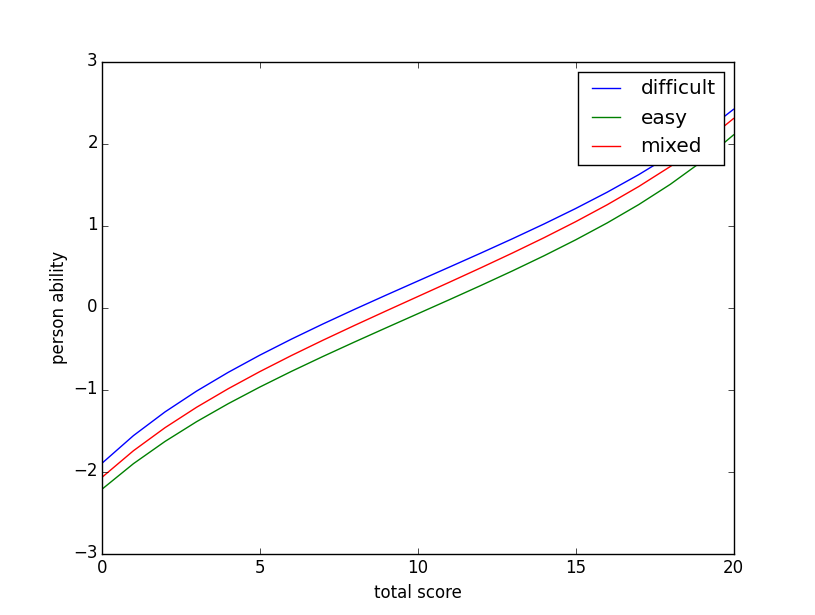
\includegraphics[height=1.5in]{scoring.png}
\end{figure}

  \end{frame}
  \begin{frame}
    
    上图中三组数据分别是20个难题,20个容易题,和10个难题和10个容易题的混合组,
由上图可看出每一条曲线有如下特点:
\begin{enumerate}
\item{能力和分数的关系在高分和低分段斜率比较大,非线性性比较明显,而在中部接近线性。}
\item{平均水平能力为0对应答出来一半的题目,曲线具有对称性。}
\end{enumerate}•
比较不同的曲线也符合直观,答出同样数量的题,对于难题组能力高,混合组能力次之,最末为简单题组。
通过用Ability而不是score来衡量从而消除了某一次Test题目的影响而在一个统一的scale上比较。
\end{frame} 
   \begin{frame}
    
    \frametitle{精度分析}
对于单次测试而言,可以用总的Fisher信息量$I(\beta)$衡量精度,一般而言,对于某一个估计的值$\hat{\beta}$,$I(\hat{\beta})$越大则表明
估计统计量的方差越小,能力估计的精度越高。[\ref{A4}]
基于MLE的方法一般都是有偏的,即估计统计量$\hat{\beta}$的均值不等于$\beta$,由于引入了先验的分布,这种偏差在两级状态会非常明显。
[\ref{A5}],
下图是比较两组题目bias的结果:
\begin{figure}[!ht]
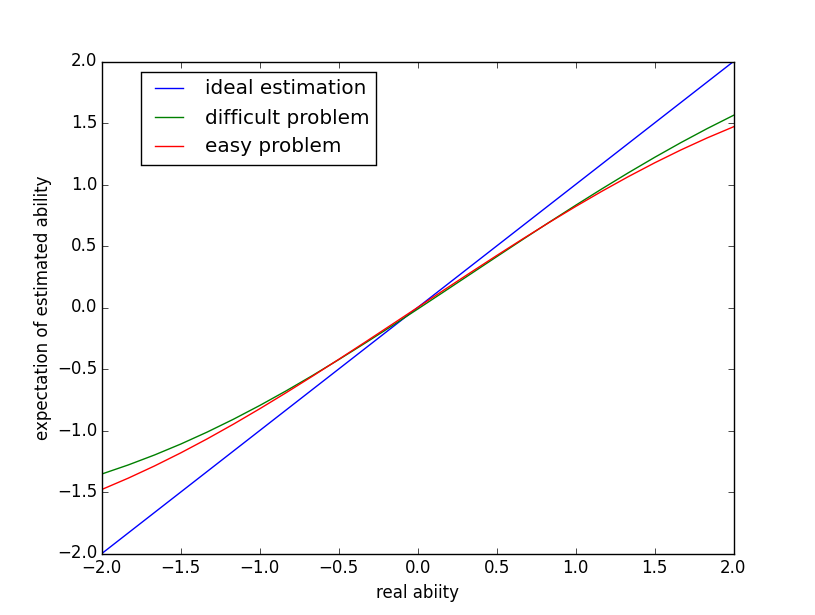
\includegraphics[height=1.5in]{bias.png}
\end{figure}
  \end{frame} 
   \begin{frame}
    
    如果person的能力接近平均水平(ability $\approx$ 0),则几乎没有bias,但两级的bias会比较大。由于采用了先验的正态总体假设,对于高分,会低估person的能力而对于低分则会高估person的能力。如果题目较难,高分段的bias减小而低分段的bias增大。

  \end{frame}

  \appendix
   \begin{frame}
    \label{A3}
    用$\beta$表示某人的能力,$\beta$的先验分布记成
$p(\beta)$,一般是正态分布,表示在没有考试成绩的时候对其能力的估计,设此人参加了有$i=1,2,..I$个item组成的测试,得分为$x_i$,
每道题的难度为$\delta_i$,由贝叶斯公式,对其成绩的后验估计为:
\pause\begin{equation}
p(\beta|\vec{x})=\frac{p(\beta)p(\vec{x}|\beta)}{p(\vec{x})}\propto p(\beta)p(\vec{x}|\beta)
\end{equation}
$\beta$最有可能的取值为:
\pause\begin{equation}\label{eq:map}
\argmax_{\beta} p(\beta)p(\vec{x}|\beta)
\end{equation}
其中$p(\vec{x}|\beta)$由Rasch Model给出:
\pause\begin{equation}
p(\vec{x}|\beta)=\prod_{i=1}^I \frac{exp(x_i(\beta-\delta_i))}{1+exp(\beta-\delta_i)}
\end{equation}
  \end{frame}
   \begin{frame}
    
对含先验分布的对数似然函数
$\log(p(\vec{x}|\beta))$关于$\beta$求导得:
\pause\begin{equation}\label{eq:score}
\frac{p'(\beta)}{p(\beta)}+\sum_{i=1}^I x_i =\sum_{i=1}^I \frac{exp(\beta-\delta_i)}{1+exp(\beta-\delta_i)}
\end{equation}
上面方程的解$\beta$对各项得分的依赖仅仅通过总分$\sum_{i=1}^I x_i$的形式,因此总分是参数$\beta$的充分统计量。由于Rasch  dichotomous Model对person的能力只有一个维度的假定,在items一定的情况下,相同能力与相同总分一一对应。
如果不加先验分布,在全对和全错两种极端情况下方程(\ref{eq:score})无解,因此适当的先验分布是必要的,有用户ability数据的情况下可以拟合正态分布的参数,在缺少用户数据的初始化阶段可以用标准正态分布代替,此时上式第一项化为$-\beta$。

  \end{frame}
   \begin{frame}\label{A4}
    
    \frametitle{Rasch模型Fisher信息量}
    $I(\beta)$的计算公式为:
\begin{equation}
I(\beta)=-E(\frac{\partial^2 \log p(\vec{x}|\beta)}{\partial \beta^2})
\end{equation}
对于Rasch Model,代入似然函数表达式,取先验分布为正态分布,则有
\begin{equation}
I(\beta)=1+\sum_{i=1}^I \frac{exp(\beta-\delta_i)}{(1+exp(\beta-\delta_i))^2}
\end{equation}
上式中第一项是先验分布的信息量,后面分别是每一个item的信息量(item infromation function),它们彼此独立因而可以相加。上式的和也被称为
Test Information Function(TIF).

  \end{frame}
   \begin{frame}
    
    对于每一个item,其IIF有左图所示的形式:
    \begin{figure}
 \begin{subfigure}{.5\textwidth}
  \centering
  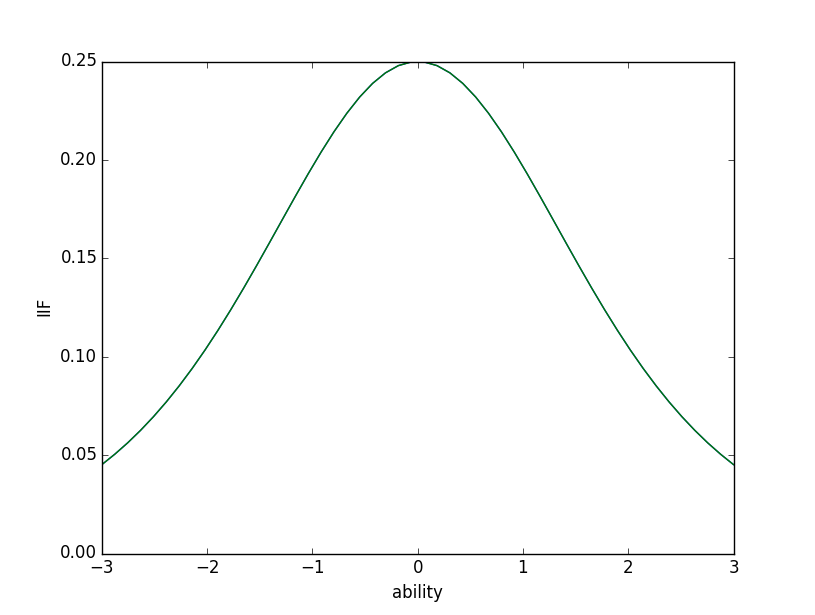
\includegraphics[height=1.5in]{IIF.png}
 \end{subfigure}%
\begin{subfigure}{.5\textwidth}
  \centering
  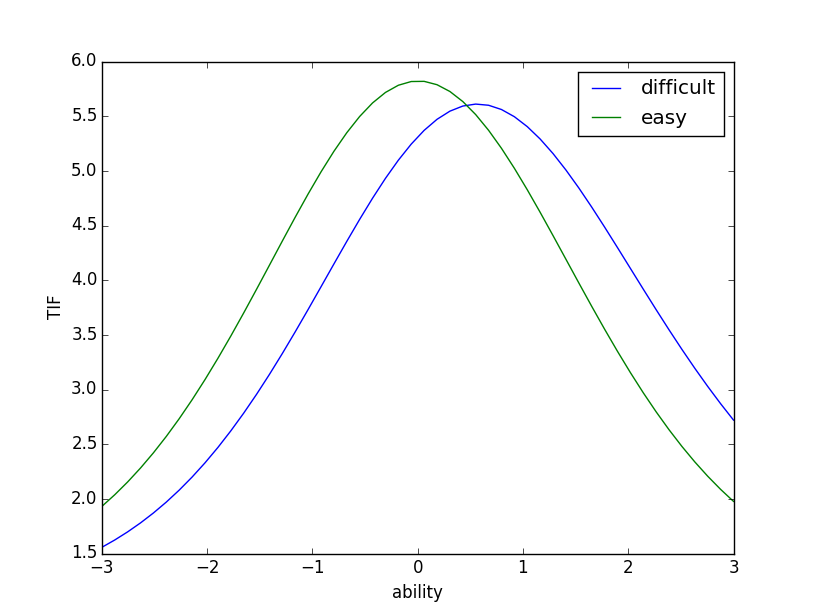
\includegraphics[height=1.5in]{TIF.png}
 \end{subfigure}
\end{figure}

左图是假定item difficulty为0,当$\beta-\delta_i>3$时(题目过难或过易),IIF已经小于0.05,在这种情况下能力估计的误差为比较大。
由于先验分布对TIF的贡献是常数,可以在一定程度上减轻能力的极端情况造成的信息量过少的问题。 右图是20道题的TIF结果,对于难题组,全对的信息量要比简单题大,而全错的信息量比简单题小,这符合一般经验。

  \end{frame}

   \begin{frame}\label{A5}
    计算bias需要计算给定真实能力后计算关于估计量的期望值,在对模型没有任何了解的情况下可以采用Monte Carlo模拟,但对于
Rasch Model由(\ref{eq:score})式得$r_I=\displaystyle\sum_{i=1}^I x_i$是$\beta$的充分统计量,于是首先计算总分$r_I$的分布,
再由
\begin{equation}
E(\hat{\beta}(r_I))=\sum_{i=1}^I \hat{\beta}(i)P(r_I=i)
\end{equation}
计算出期望值。在上式中$\hat{\beta}(i)$可以通过对(\ref{eq:map})求解极大值得到,而$r_I$的分布可以类比组合数的计算方法递推得到。
记$A_n^k=\displaystyle\sum_{k=1}^n x_k$,则有如下递推公式:
    \frametitle{Rasch模型Bias数值计算}
  \end{frame}
   \begin{frame}
\begin{equation}
A_n^k=P(x_n=1)A_{n-1}^{k-1}+P(x_n=0)A_{n-1}^k
\end{equation}
上式中$P(x_n=1)$为第n道题的答对概率。
该方法计算规模为$O(n^3)$,其中n为item 数量,相比Monte Carlo模拟需要大量重复才能得到比较精确的结果在n不大时效率比较高。
\end{frame}
% etc
   \begin{frame}[allowframebreaks]
  \frametitle<presentation>{Further Reading}    
  \begin{thebibliography}{10}    
  \setbeamertemplate{bibliography item}[online]
  \bibitem{Autor1990}
    \newblock {\em Rasch model estimation}.
    \newblock https://en.wikipedia.org/wiki/Rasch\_model\_estimation
   \setbeamertemplate{bibliography item}[article]
  \bibitem{Jemand2000}
   Patrick Mair,Reinhold Hatzinger,Marco J. Maier
    \newblock Extended Rasch Modeling: The R Package eRm.
  \end{thebibliography}
\end{frame}
\end{document}